\begin{center}
\footnotesize\noindent\fbox{
	\parbox{\textwidth}{
Verificato che la funzione \(f(x_1,x_2) = x_1^2+x_2^3-x_1x_2\) ha un punto di minimo relativo in (1/12, 1/6), costruire una tabella in cui si riportano il numero di iterazioni eseguite, e la norma euclidea dell'ultimo incremento e quella dell'errore con cui viene approssimato il risultato esatto utilizzando la function sviluppata al punto precedente per valori delle tolleranze pari a \(10^{-t}\), con t = 3,6. Utilizzare (1/2, 1/2) come punto di innesco. Verificare che la norma dell'errore \'e molto pi\'u piccola di quella dell'incremento (come mai?)
	}
}\end{center}

\noindent Si verifica innanzitutto analiticamente l'esistenza di un punto di minimo relativo in \((\frac{1}{12}, \frac{1}{6})\) considerando il sistema non lineare:
\[
F(\vec{x}) = \vec{0} \quad \text{con} \quad F = \begin{bmatrix}\frac{\partial}{\partial x_1}f(x_1,x_2) \\ \frac{\partial}{\partial x_2}f(x_1,x_2)  \end{bmatrix}
\]
\[
\frac{\partial}{\partial x_1}f(x_1,x_2) = 2x_1 -x_2 \quad \frac{\partial}{\partial x_2}f(x_1,x_2) = 3x_2^2 - x_1
\]
\[
\begin{cases}
2x_1 -x_2 = 0 \\
3y^2 - x_1 = 0
\end{cases}
\quad \text{ha come soluzioni} \quad \begin{bmatrix}0 & 0 \end{bmatrix} \quad \text{e} \quad \begin{bmatrix}\frac{1}{12} & \frac{1}{6}\end{bmatrix}
\]
\\
\noindent I punti trovati sono quindi punti stazionari della funzione data. Si consideri ora la matrice Hessiana della funzione \(f(x,x_2)\), che coincide con la matrice Jacobiana della funzione \(F\):
\[
H =
\begin{bmatrix} f_{x_1x_1} & f_{x_1x_2} \\ f_{x_2x_1} & f_{x_2x_2} \end{bmatrix}
=
\begin{bmatrix} 2 & -1 \\ -1 & 6x_2 \end{bmatrix}
= J_F
\quad
\det(H) = 12x_2 - 1
\]

\noindent Il determinante dell'Hessiana \'e positivo per \(x_2=\frac{1}{6}\), ed il primo elemento \'e positivo: abbiamo un punto di minimo relativo in \((\frac{1}{12}, \frac{1}{6})\).
\\
\\
\noindent Per avere una ulteriore conferma visiva, \'e stata definita la seguente funzione \(\overline{f}(x_1,x_2)\):

\[
f(\frac{1}{12}, \frac{1}{6}) = -\frac{1}{432} \quad \overline{f}(x_1,x_2) = f(x_1,x_2) + \frac{1}{432} \quad \text{in modo che} \quad \overline{f}(\frac{1}{12}, \frac{1}{6}) = 0
\]
\\

\noindent Si \'e quindi studiato il segno di \(\overline{f} \) con il seguente codice Matlab con cui \'e stato prodotto il plot 3D mostrante il comportamento di \(\overline{f} \) in un intorno di \((\frac{1}{12}, \frac{1}{6})\):
\\
\lstinputlisting[language=Matlab]{cap3/3_11_sign.m}

\begin{center}
	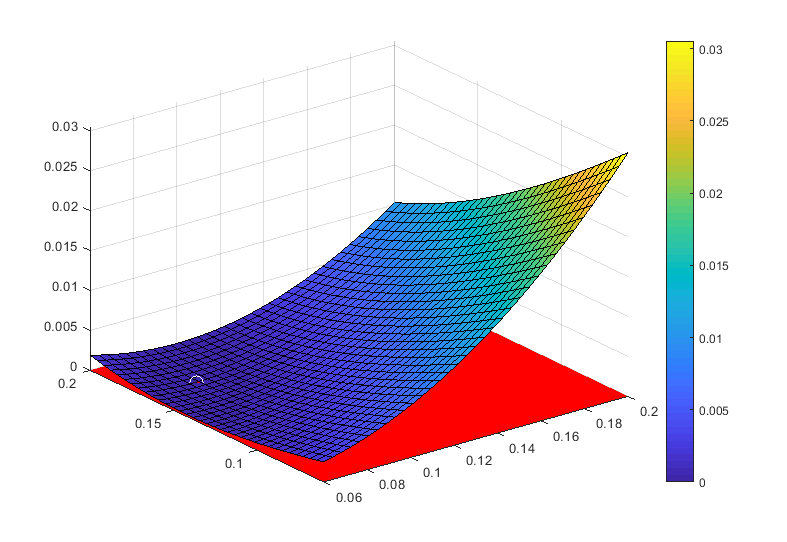
\includegraphics[scale=0.7]{cap3/3_11_sign.png}
\end{center}

\noindent Poich\'e \(\overline{f}\) \'e tutta positiva in un intorno di \((\frac{1}{12}, \frac{1}{6})\) e pari a zero solo in quel punto, possiamo concludere che \((\frac{1}{12}, \frac{1}{6})\) \'e sicuramente un minimo relativo di \(f\).
\\
\\
\noindent Per quanto riguarda l'utilizzo del metodo di Newton, \'e stata scritta una versione modificata della function dell'Esercizio precedente per restituire i dati da mostrare nella tabella richiesta.
\\
\\ RIFARE I CONTI
\\
\lstinputlisting[language=Matlab]{cap3/3_11.m}

\begin{tabular}{l*{15}{c}}
 toll. & \vline& it. & \vline& \(x_1\) &\vline& \(x_2\) & \vline& norma ultimo incr. & \vline& norma errore\\
\hline
 \(10^{-3}\) & \vline& 10 & \vline& 0.083577& \vline& 0.16715 &\vline& 0.77204 \(\times 10^{-3}\) & \vline& 0,54128 \(\times 10^{-3}\) \\
 \(10^{-4}\) & \vline& 13 & \vline& 0.083364& \vline& 0.16673 &\vline& 9.6505 \(\times 10^{-5}\) & \vline& 7,03673 \(\times 10^{-5}\) \\
 \(10^{-5}\) & \vline& 17 & \vline& 0.083335& \vline& 0.16667 &\vline& 6.0316 \(\times 10^{-6}\) & \vline& 3,72678 \(\times 10^{-6}\) \\
 \(10^{-6}\) & \vline& 20 & \vline& 0.083335& \vline& 0.16667 &\vline& 6.0316 \(\times 10^{-6}\) & \vline& 3,72678 \(\times 10^{-6}\) \\
\end{tabular} \\
\\
\noindent Come si pu\'o notare, la norma dell'errore (ovvero \(||x - \overline{x}||\) con \(\overline{x} = [\frac{1}{12}, \frac{1}{6}]^T\)) \'e pi\'u piccola di quella dell'ultimo incremento.

